\section{Experimental Apparatus}
The experiment was carried out at the Idaho Accelerator Center, using their short pulsed linear accelerator.
The accelerator is a radio frequency accelerator operating at the L--band frequency of 1300 MHz.
It is capable of pulse widths ranging from 50 ps to 2 $\mu$s with a maximum energy of 44 MeV.
See figure~\ref{fig:Facility} for a top down schematic of the entire experimental arrangement.
\begin{figure}[h]
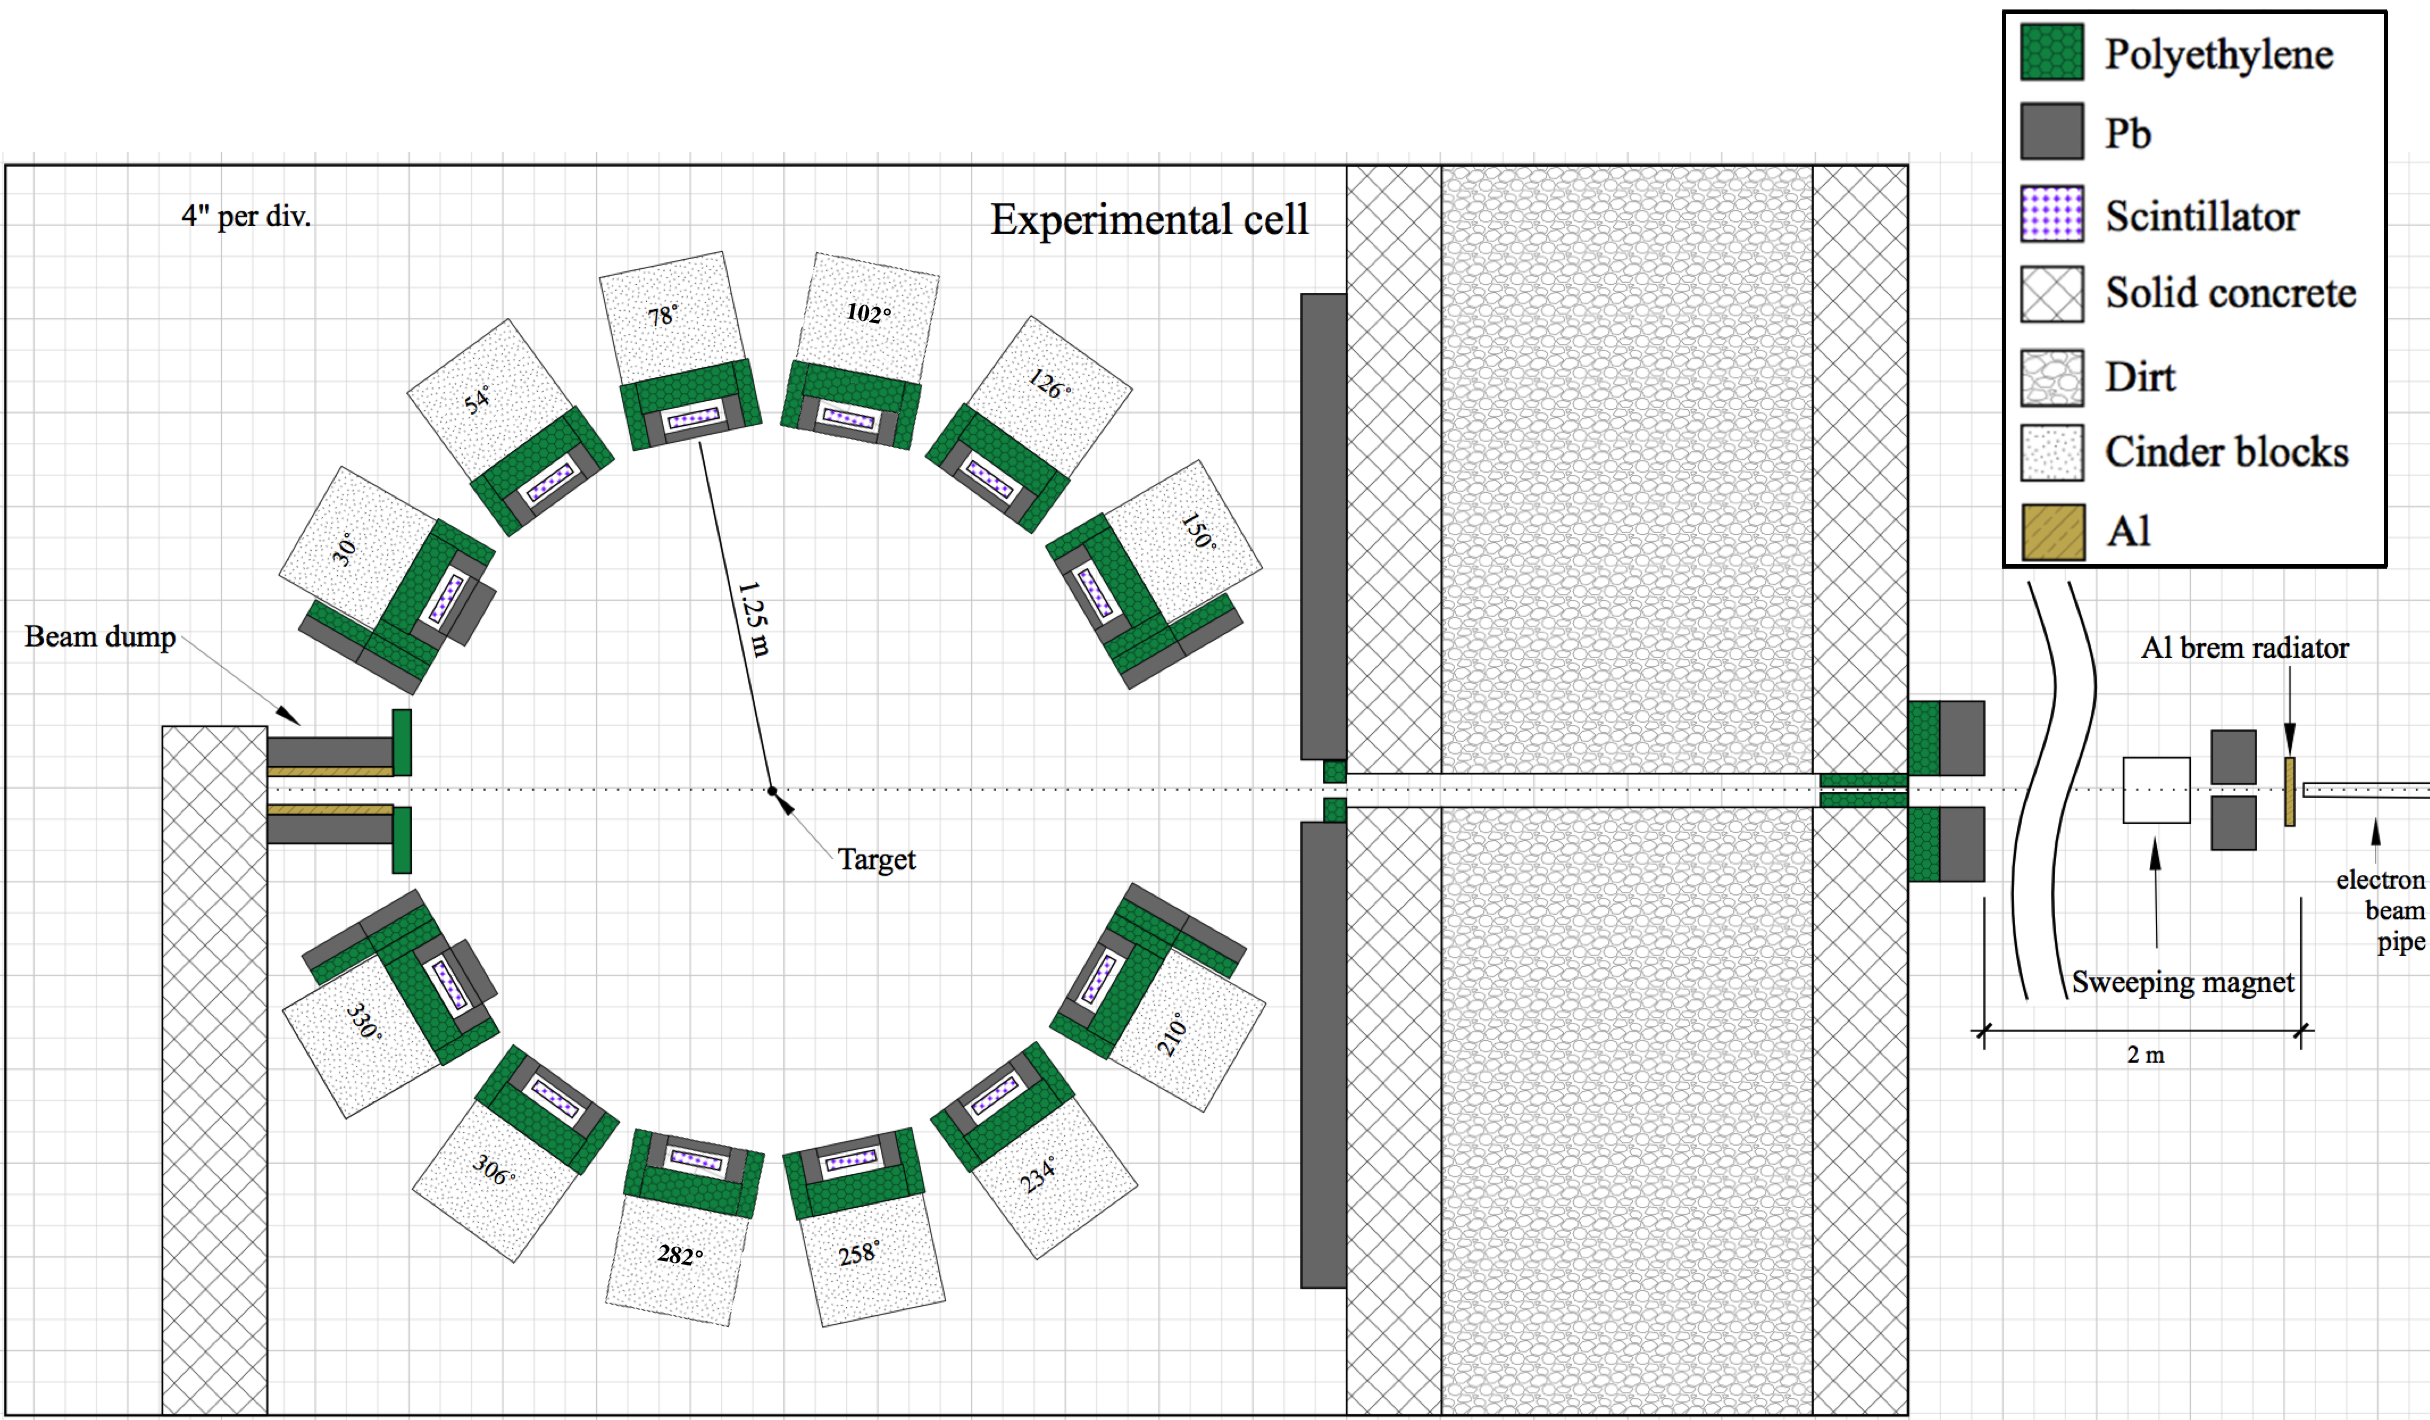
\includegraphics[width=\textwidth]{Content/Methods/ExpArangment.png}
\caption{To-scale top down schematic of the entire experimental setup.
The detectors supporting structures are each labeled with a degree value.
The degree corresponds to the angle of the detector from the direction of the beam.
For a better perspective of the scintillation cells alone, see ~\ref{fig:DetGeom}}
\label{fig:Facility}
\end{figure}

\subsection{Detectors}
\label{section:Detectors}
\begin{figure}[h]
\centering
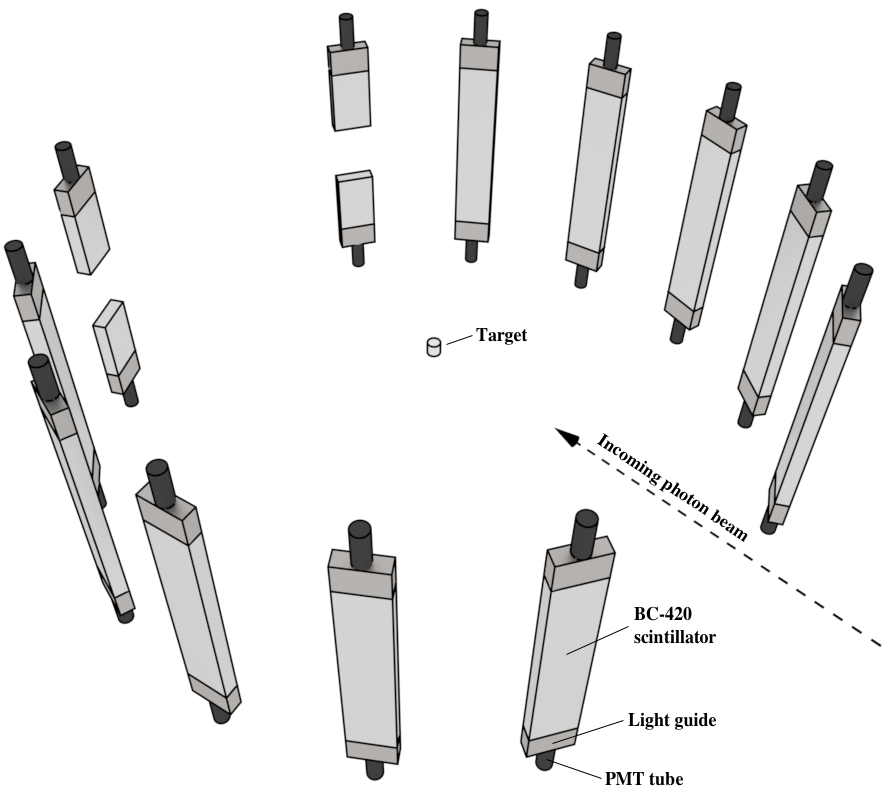
\includegraphics[width=0.95\textwidth]{Content/Methods/Detectors.png}
\caption{3D-rendering of the bare scintillation cells showing how the detectors are positioned in space.
Each detector is fully enclosed in a shielding structure, which is not shown in this depiction.}
\label{fig:DetGeom}
\end{figure}
The neutron detector array consists of fourteen cells made from Polyvinyl Toluene (PVT), a type of organic plastic scintillator, acquired from the Transportation Security Administration (TSA) as surplus.
The scintillation cells were arranged in a ring around the target (see figure ~\ref{fig:DetGeom}).
Each scintillator is instrumented with two Hamamatsu 580-17 photomultiplier (PMT) tubes, one fixed on each end.
A 10 cm block of a non-scintillating material, serving as a light guide, was fixed between each PMT and scintillator.
The light guides back the PMTs off from the scintillator so that scintillation light produced near a corner of a scintillator has a line of sight to the PMT nearest to the corners.
Micro imperfections on the surface of the scintillation cells were reduced through polishing in order to increases the chance that scintillation light remains in the cell due to total internal reflection.
The cells were then wrapped in reflective Tyvek.

Two different detector designs had to be used in order to address a high rate of gammas on the detectors located furthest downstream of the beam.
Ten of the fourteen detectors did not have this problem, and have dimensions of 76.2X15.2X3.8 cm$^3$.
The remaining four had their dimensions reduced to 25.4X15.2X3.8 in order to address excessively high gamma detection rates, which are a result of the forward scattering of photons from the target.
High gamma detection rates lead to high levels of dead-time and therefore a reduction in neutron efficiency.
Prior to this modification, the gamma detection rate was nearly 1.0 per pulse in each.
After the modification, the gamma detection rate fell to 0.5 gammas per pulse, leading to a net increase in neutron detection efficiency.
The detectors at \pm$30 degrees also differ from the rest because they were instrumented with only a single PMT .

The location of a particle hit along the detector's 30 inch length is determined by the timing difference between signals in the top and bottom PMT .
This method uses the fact that the scintillation light travels at a constant speed through the cell.
This technique is not possible for the four the downstream detectors at $\pm 30^{\circ}$, since these have only a single PMT.
For these detectors, particle position is assumed to be at the middle of the cell.
For further detail on particle position reconstruction, see section ~\ref{reconstruction}.

\subsection{Data Acquisition}
A data acquisition system based on NIM/VME standard was used.
A wiring diagram is shown in figure~\ref{fig:WiringDiagram}.
The PMTs are supplied voltages ranging from 1300 to 1500 V by a Locroy 1458 high voltage mainframe.
Analogue signals from the PMTs are fed into a leading edge discriminator with input thresholds ranging from 30 mV to 50 mV .
The logic signals from the discriminator are then converted to ECL logic and fed into a CAEN model V1290A TDC .
The timing of signals from the PMTs are always measured relative to a signal from the accelerator provided at the beginning of each pulse.
On the software side, the CODA software package developed by Jefferson Lab was used to carry out the acquisition of data from the TDC and to convert the it into a usable format.
\begin{figure}[h]
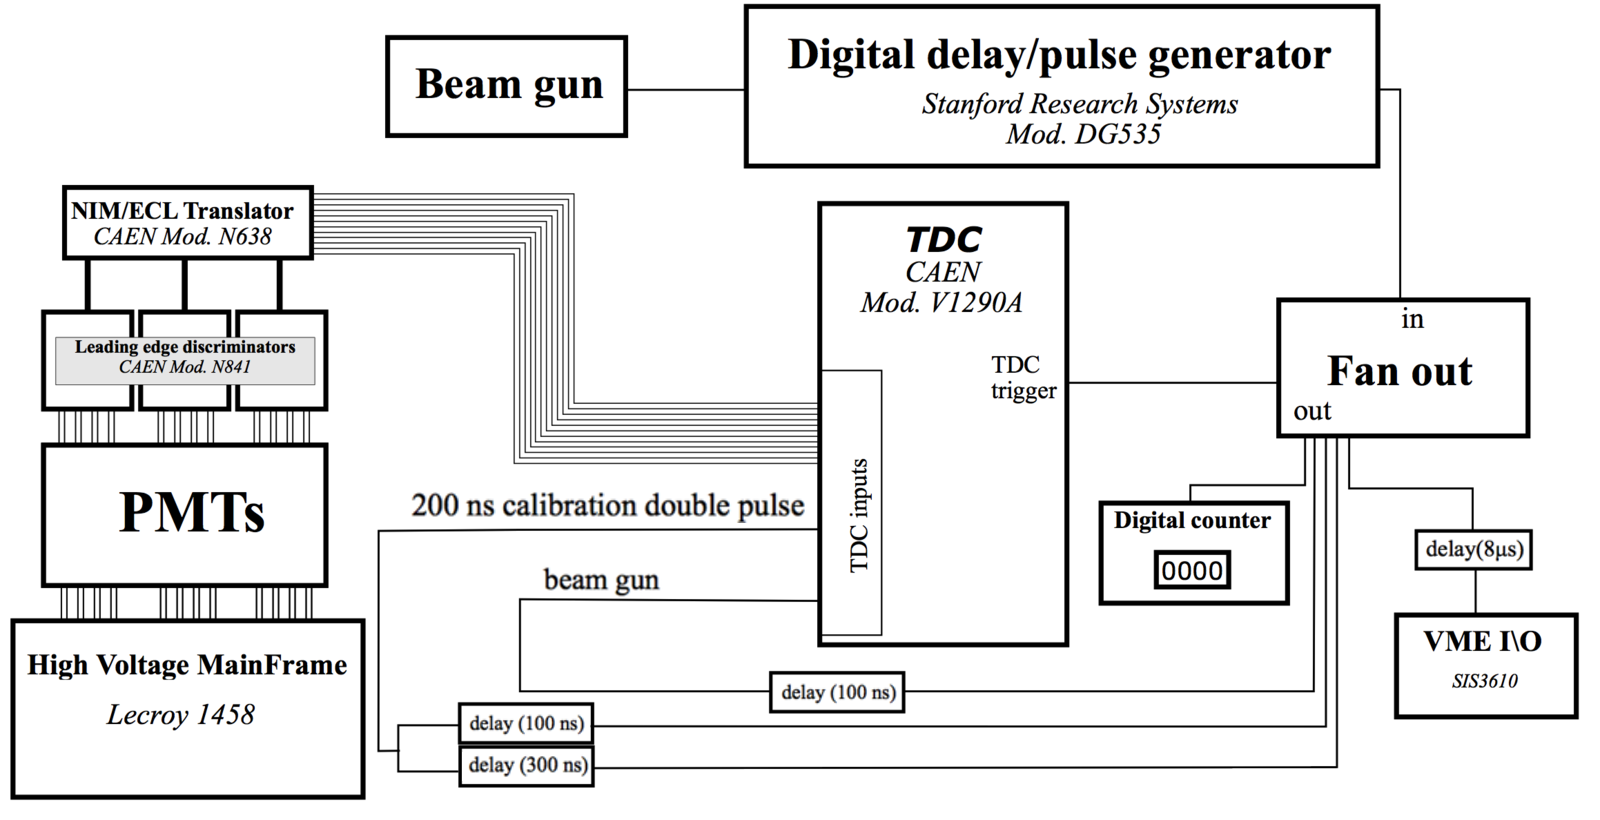
\includegraphics[width=\textwidth]{Content/Methods/WiringDiagram.png}
\caption{Wiring diagram of the electronics setup. }
\label{fig:WiringDiagram}
\end{figure}